%!TEX root = ../report.tex

\chapter{Further details regarding the Dataset}\label{appendix:dataset}

\section{Selection of a labeling tool}

\textbf{[Incomplete]}

In order to reduce the time required to annotate an image, it was imperative to select a tool which is specifically designed for semantic segmentation and also provides algorithms which helps the annotator by providing labeling automation to the highest possible extent.

The following available tools were evaluated for ease of use and time taken for annotation:
	\begin{itemize}
		\item LabelMe: web based tool is public and data would also be public.
		\item LabelMe Matlab toolbox: yet to try..
		\item University bonn annotation tool:
		\item Pixel annotation tool (using watershed algorithm): works in windows. Seems to be useful.
		\item Ratsnake: tool dint seem to be useful although the website had options like superpixel suggestions.
		\item LabelImg: Can be used but time consuming.
		\item Figi: used in medical image segmentation. Has many options. Still exploring.
		\item Supervisely.
		\item MATLAB ImageLabeler available in release R2017b (Computer Vision Toolbox).
	\end{itemize}

\section{Description of the labeling process}
\label{section:process}
MATLAB ImageLabeler was used for the labeling process. At first, label definitions are created and exported to a .mat file. This file is used to load label definitions for all images to maintain consistency of labels. The contents of the .mat file is shown in the Figure \ref{Fig:labeldef}.
	
	\begin{figure}
		\begin{subfigure}{.5\textwidth}
			\centering
			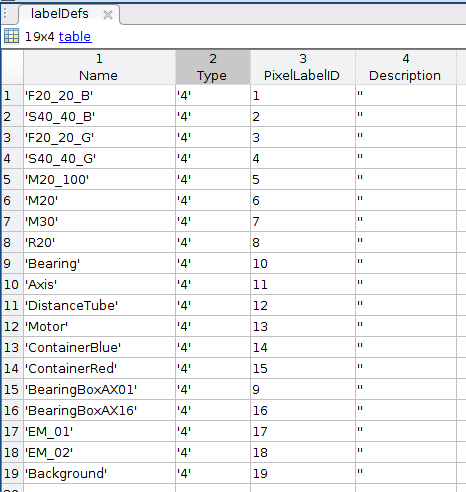
\includegraphics[width=1\linewidth]{images/labelDef}
			\caption{}
			\label{Fig:labeldef}
		\end{subfigure}
		\begin{subfigure}{.5\textwidth}
			\centering
			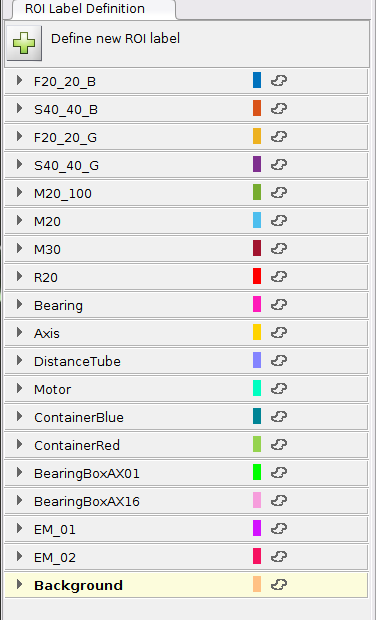
\includegraphics[width=0.83\linewidth]{images/roi_label_defintions}
			\caption{}
			\label{Fig:ROI}
		\end{subfigure}
		\caption{(a) Contents of the labelDefs .mat file, (b) ROI Label Definitions window.}
		\label{Fig:def_ROI}
	\end{figure}
	
The ImageLabeler app, by default, provides different tools which help create pixelwise labels. The tools are shown in the Figure \ref{Fig:IL_tools}. These tools become accessible once an image and the label definitions are loaded. A short description of the tools is given below:
	\begin{figure}
		\centering
		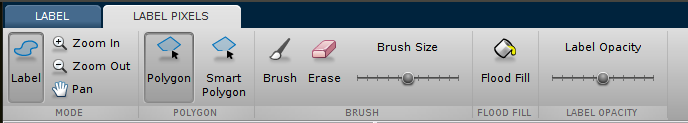
\includegraphics[scale=0.55]{images/label_tools}
		\caption{Tools provided by the ImageLabeler app}
		\label{Fig:IL_tools}
	\end{figure}
	
	\begin{itemize}
		\item Polygon: This can be used to trace an object boundary by placing dots. Once a closed contour is created, pixels within the contour get assigned the corresponding object label.
		\item Smart Polygon: Can be used in a similar fashion like the Polygon tool. This tool, in addition, tries to reach out to the nearby edges of the drawn polygon.
		\item Brush and Erase: Square shaped brush and eraser to either label a region or remove labels from a region. The size of the square can be changed by using the Brush Size slider.
		\item Flood Fill: This tool provides same labels to pixels which are similar in terms of the intensity with the selected pixel.
		\item Label Opacity: This tool provides a sliding bar which varies the opacity of the overlayed labels on the image. This is helpful to visualize the assigned labels.
		\item Zoom In, Zoom Out, Pan: These tools improve the ease of labeling by providing means to focus on particular regions by zooming and panning.
	\end{itemize}
	
The ImageLabeler app by default assigns different colors to different objects to aid visualization. The label colors are shown in the ROI Label Definition window shown in Figure \ref{Fig:ROI}. An example of an object in the ImageLabeler tool once the annotation is complete is shown in Figure \ref{Fig:ex_ann}.
	
	\begin{figure}
		\centering
		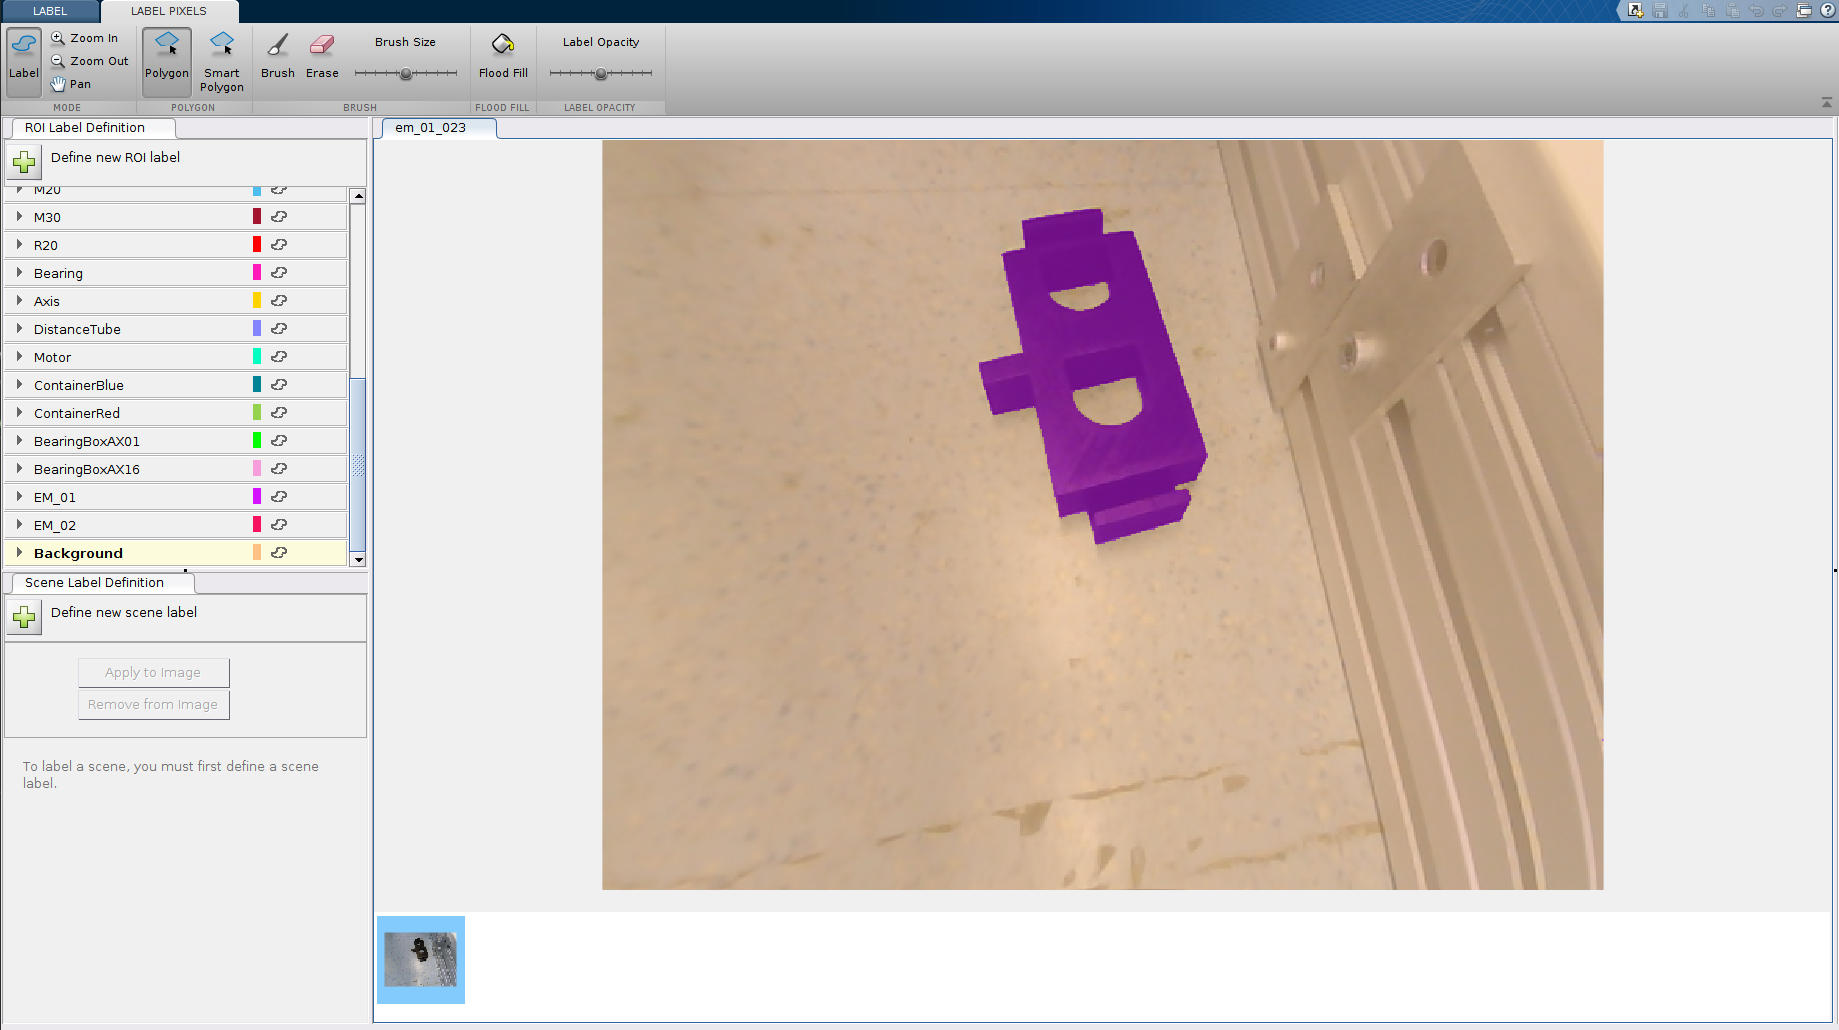
\includegraphics[scale=0.2]{images/imglabler_eg}
		\caption{An object labeled in the ImageLabeler.}
		\label{Fig:ex_ann}
	\end{figure}
	
The ImageLabeler app does not provide any tool to label all unlabeled pixels as background. In order to save time, the following workarounds have been used:
	\begin{itemize}
		\item The images taken for the dataset each have only one object in them.
		\item Only the object region is labeled.
		\item Since the ImageLabeler app does not provide any tool to label all unlabeled pixels as background, a python code which simply reads the label image and replaces unlabeled values 0 with background label value 19, was used for this purpose. The code is also used to double check the label image in order to avoid noisy labeling.
	\end{itemize}
	
The Export Labels --$>$ To File option can be used to save the annotations. This is done for all images individually to arrive at the folder structure shown in Figure \ref{Fig:fsa}.
	
The saved .mat file can be loaded into ImageLabeler again to further modify labels if required later. The 'Label\_1.png' file located in the PixelLabelData folder (as can be seen in Figure  \ref{Fig:fsa}) is the label image. This image is renamed to have the same name as the image file and a folder structure as in Figure  \ref{Fig:fsb} is created by using a python code.
	
\begin{center}
	\begin{figure}
		\begin{subfigure}{.5\textwidth}
			\centering
			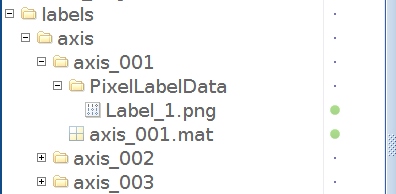
\includegraphics[width=1\linewidth]{images/folder_structure}
			\caption{Folder structure of saved labels}
			\label{Fig:fsa}
		\end{subfigure}
		\begin{subfigure}{.5\textwidth}
			\centering
			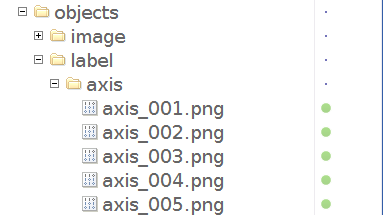
\includegraphics[width=1\linewidth]{images/folder_structure_aug}
			\caption{Rearranged folder structure}
			\label{Fig:fsb}
		\end{subfigure}
		\caption{Different folder structures}
		\label{Fig:fs}
	\end{figure}
\end{center}

The final folder structure is shown in Figure \ref{Fig:fsil}. The image folder and label folder are similar and contain object images and corresponding label images with same names.

\begin{center}
	\begin{figure}
		\begin{subfigure}{.5\textwidth}
			\centering
			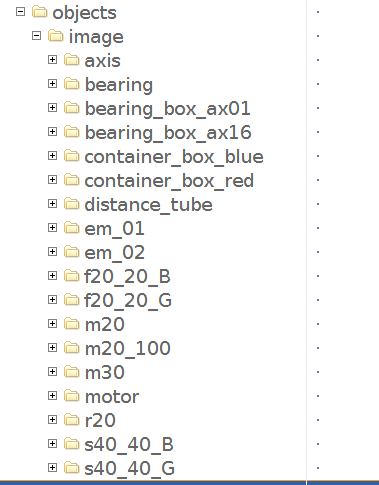
\includegraphics[width=.7\linewidth]{images/folder_image}
			%\caption{}
			\label{Fig:fsila}
		\end{subfigure}
		\begin{subfigure}{.5\textwidth}
			\centering
			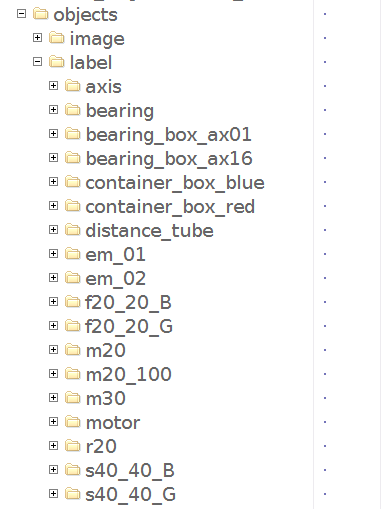
\includegraphics[width=.7\linewidth]{images/folder_label}
			%\caption{}
			\label{Fig:fsilb}
		\end{subfigure}
		\caption{Folder structure showing different object folders in both image and label folders.}
		\label{Fig:fsil}
	\end{figure}
\end{center}

\section{Search keywords for background images}

Keywords used for downloading background images are listed in Table \ref{Table:download}.

\begin{table}
	\centering
	\begin{tabular}{|c|c|c|c|c|c|c|c|}
	\hline 
    Used in & Search keyword(s) & \makecell{Number of \\images selected} \\ 
	\hline 
	Training set & \makecell{640x480 background images, \\640x480 textures images, \\640x480 wallpapers} & 150 \\ 
	\hline 
	Validation set & 640x480 abstract & 25 \\ 
	\hline 
	Test set & 640x480 paintings & 25 \\ 
	\hline 
	Shades of white & \makecell{640x480 white abstract, \\640x480 white backgrounds, \\640x480 white textures, \\640x480 white wallpaper, \\light gray, white, white clouds, \\white floors, white frost, white mist, \\white pebbles, white snow, \\white table textures} & 150 \\ 
	\hline 
	\end{tabular}
	\caption{This table lists the keywords used to download images used as background for artificial image generation.} 
	\label{Table:download}
\end{table}

\section{Generator option details}

Further details regarding the generator options used to configure the artificial image generation algorithm is given in Table \ref{Table:govals}.

\begin{table}
\centering
\begin{tabular}{|c|c|c|c|c|c|c|c|}
\hline 
\textbf{Generator options} & Default value & \makecell{Is required?} \\ 
\hline 
\textbf{mode} & \makecell{1} & \makecell{Not required} \\ 
\hline 
\textbf{image\_dimension} & \makecell{[480, 640]} & \makecell{Not required} \\ 
\hline 
\textbf{num\_scales} & \makecell{'randomize'} & \makecell{Not required} \\ 
\hline 
\textbf{backgrounds\_path} & \makecell{None} & \makecell{Required if mode is 1} \\ 
\hline 
\textbf{image\_path} & \makecell{-} & \makecell{Required} \\ 
\hline 
\textbf{label\_path} & \makecell{-} & \makecell{Required} \\ 
\hline 
\textbf{obj\_det\_label\_path} & \makecell{None} & \makecell{Required if save\_label\_preview \\is True and mode is 2} \\ 
\hline 
\textbf{real\_img\_type} & \makecell{'.jpg'} & \makecell{Not required} \\ 
\hline 
\textbf{min\_obj\_area} & \makecell{20} & \makecell{Not required} \\ 
\hline 
\textbf{max\_obj\_area} & \makecell{70} & \makecell{Not required} \\ 
\hline 
\textbf{save\_label\_preview} & \makecell{False} & \makecell{Not required} \\ 
\hline 
\textbf{save\_obj\_det\_label} & \makecell{False} & \makecell{Not required} \\ 
\hline  
\textbf{save\_mask} & \makecell{False} & \makecell{Not required} \\ 
\hline 
\textbf{save\_overlay} & \makecell{False} & \makecell{Not required} \\ 
\hline 
\textbf{overlay\_opacity} & \makecell{0.6} & \makecell{Not required} \\ 
\hline 
\textbf{image\_save\_path} & \makecell{None} & \makecell{Required if \\mode is 1} \\ 
\hline 
\textbf{label\_save\_path} & \makecell{None} & \makecell{Required if \\mode is 1} \\ 
\hline 
\textbf{preview\_save\_path} & \makecell{None} & \makecell{Required if \\save\_label\_preview is True} \\ 
\hline 
\textbf{obj\_det\_save\_path} & \makecell{None} & \makecell{Required if \\save\_obj\_det\_label is True} \\ 
\hline 
\textbf{mask\_save\_path} & \makecell{None} & \makecell{Required if \\save\_mask is True} \\ 
\hline 
\textbf{overlay\_save\_path} & \makecell{None} & \makecell{Required if \\save\_overlay is True} \\ 
\hline 
\textbf{start\_index} & \makecell{0 if mode is 1 \\ '' if mode is 2} & \makecell{Not required} \\ 
\hline 
\textbf{name\_format} & \makecell{'\%05d'} & \makecell{Not required} \\
\hline 
\textbf{remove\_clutter} & \makecell{True} & \makecell{Not required} \\
\hline 
\textbf{num\_images} & \makecell{20} & \makecell{Not required} \\ 
\hline 
\textbf{max\_objects} & \makecell{10} & \makecell{Not required} \\ 
\hline 
\textbf{num\_regenerate} & \makecell{100} & \makecell{Not required} \\ 
\hline 
\textbf{min\_distance} & \makecell{100} & \makecell{Not required} \\ 
\hline 
\textbf{max\_occupied\_area} & \makecell{0.8} & \makecell{Not required} \\ 
\hline 
\textbf{scale\_ranges} & \makecell{None} & \makecell{Not required} \\ 
\hline 
\end{tabular}
\caption{Default value of generator options and whether the options are required to be set.}
\label{Table:govals}
\end{table}

\chapter{Sample predictions}
Your first appendix

\chapter{Hyperparameters}
Your second chapter appendix
